\section{Study design}
\textbf{Model, tasks, and Study A.} All runs use self-hosted Gemma 4 31B QAT on H200 GPUs (RTX 5090 for subagent ablations) (32k context, 4k thinking, 8k output tokens, temperature 0.2, top-p 0.95; \texttt{swegemma} 0.2.11, \texttt{adk-submission} 0.2.13) across 95 tasks from 15 repositories (54 official, 41 external). Baseline V5 allocates 480 s, 28 calls, 80 turns, and free \texttt{submit\_patch}. \textbf{Study A} (736 runs, three batches) compares V5 against a prompt policy (\texttt{v1}) requiring target counterevidence before editing and check replay afterward, plus a reuse-restricted variant (\texttt{v2}).

\textbf{Shared-draft continuation (Study B) and ablations.} \textbf{Study B} evaluates the 54 official tasks (FastAPI 26, Rich 18, Requests 9, HTTPX 1) across four batches (216 realizations, 864 sessions). Each realization generates an unfiltered draft D from V5 (240 s, 16 calls), including empty patches. A read-only constructor receives the issue and D, emits a JSON check and expected outcome, and runs it on D (30 s timeout).

\begin{figure}[htbp]
\centering
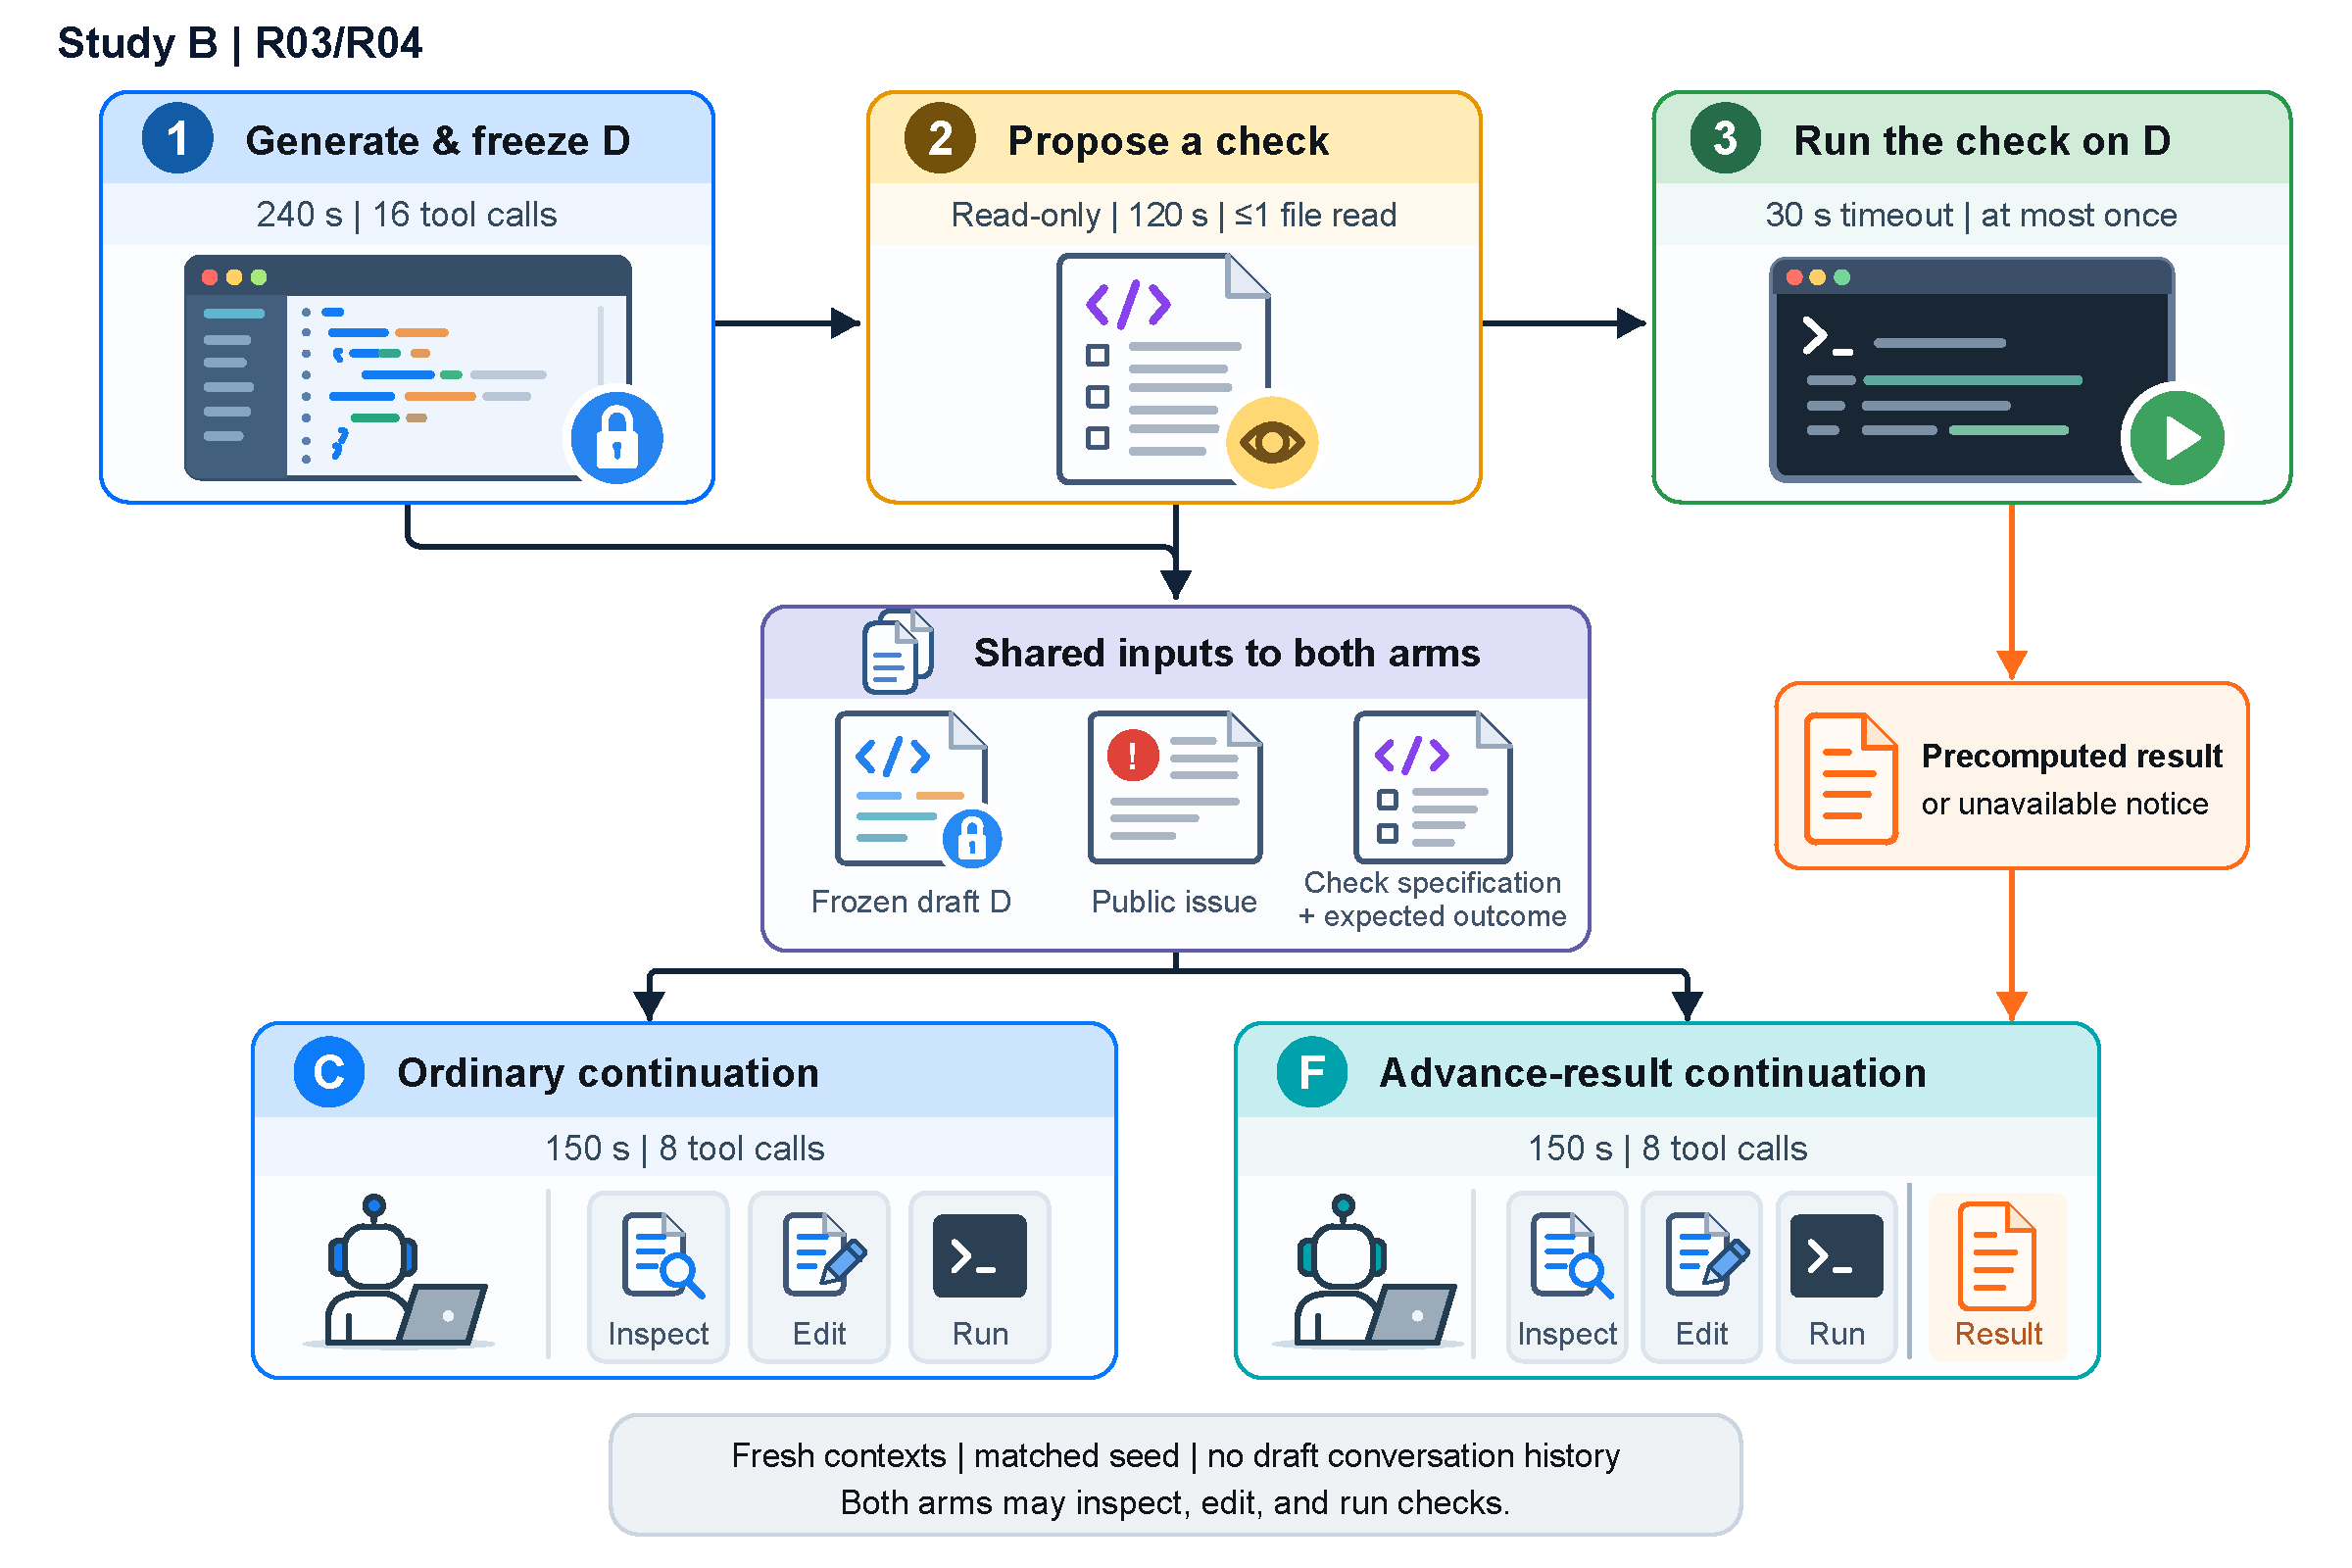
\includegraphics[width=\linewidth]{figures/study-design-v04.pdf}
\caption{Study B shared-draft design. Paired C/F continuations share code, issue text, check specifications, and budgets; only F receives the precomputed result.}
\label{fig:design}
\end{figure}

Fresh C and F continuations branch from the same D, issue, check specification, and seed without D's history (Figure~\ref{fig:design}), each receiving 150 s and 8 calls; only F receives the precomputed output. Each path totals 540 s and 26 calls in R03/R04 (R01/R02 cut constructor reads from 3 to 1 and raised time from 60 to 120 s). Three \textbf{follow-up ablations} (2,565 runs across 95 tasks) test prompt-capped subagents, schema/shell recovery, and \texttt{keep}/\texttt{reject} gates.

\textbf{Audit protocol.} Scripts extract tool sequences, stderr, \texttt{BudgetExceeded} and missing-\texttt{old\_string} rejections, malformed pagination keys, replay timing, and diffs over D across 216 packets and 432 patches (\href{supplement/reproducibility.md}{reproduction guide}). Annotations were frozen before grading; across 648 endpoints, 620 yield normal grades (five passing empty patches), 25 unknowns, and 3 unscored.
\FloatBarrier
